\chapter{Methodology}
\label{chap:ch4}

In this chapter I will describe the implementation of the three main steps taken by the engine to find the best move: generating legal moves for a position, searching for legally reachable positions from the current position, and then evaluating each one and determining which one is the best \cite{marsland1986review}.

%Description of the approach taken to build the chess engine
%Explanation of the AI techniques used and why they were chosen

\section{Move generation}
\label{sec:ch4sec1}

The engine computes the pseudo-legal moves of the pieces of the player that is moving, then it does each move, checks the state of the board, adds the move to the list of legal moves if the board is in a valid state, and then undoes the move.

To check the state of the board I used a threat map (fig. \ref{fig:threatMap}), which keeps track of the squares that are under attack or are defended by at least one piece (including empty squares, squares with allied pieces, and squares with opponent pieces). After each move, the threat map is updated in the following way: for each white piece on the board, it sets "IsAttackedByWhite" to true for all the squares it attacks, and for each black piece on the board, it sets "IsAttackedByBlack" to true for all the squares it attacks.

\begin{figure}
  \centering
  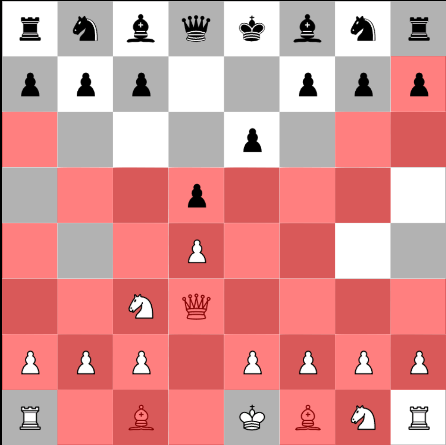
\includegraphics[scale=0.5]{figures/white-threat-map.png}
  \captionof{figure}{White threat map}
  \label{fig:threatMap}
\end{figure}

\section{Search}
\label{sec:ch4sec2}

The simplest way of searching in the game tree is through a fixed depth Minimax algorithm, which would be mathematically accurate, but would not yield good results and would be very slow. However, in combination with some optimizations and heuristics, it can compute faster and find better moves.

\subsection{Alpha-beta pruning}
\label{subsec:ch4sec2subsec1}

The Minimax algorithm was improved with Alpha-beta pruning, which preserves the accuracy of the algorithm and significantly reduces the number of nodes visited if combined with a good move ordering heuristic \cite{eric1992analysis}.

A simple pseudocode for Alpha-beta pruning is shown in fig. \ref{fig:alphabetaPseudocode}:

\begin{figure}[h]
  \centering
  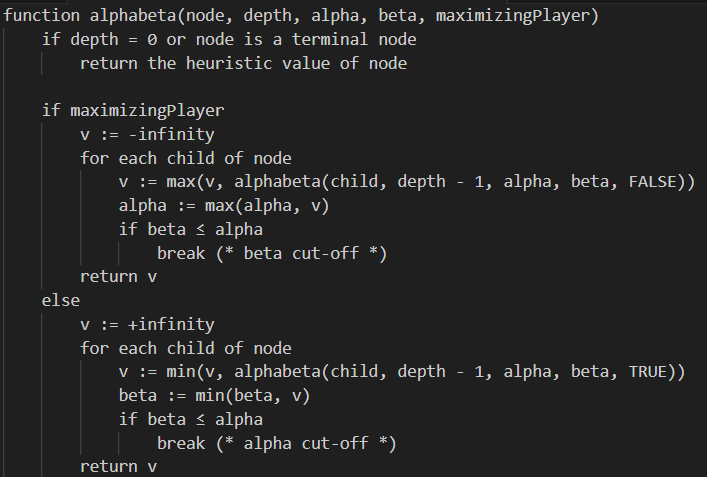
\includegraphics[scale=0.9]{figures/alphabeta-pseudocode.png}
  \captionof{figure}{Alpha-beta pruning pseudocode}
  \label{fig:alphabetaPseudocode}
\end{figure}

The heuristic I used in combination with Alpha-beta pruning is MVV-LVA (Most Valuable Victim - Least Valuable Agressor): the moves that capture pieces with high values are first, and if multiple moves capture a piece of the same value, the moves with the least valuable agressor are prioritized \cite{mvv-lva}. The heuristic is based on the observation that in chess, it is often advantageous to capture pieces of higher value than the capturing piece, while avoiding exchanges where the capturing piece is more valuable than the captured piece. It is also relatively easy to implement, and does not require much computational overhead. Other heuristics, use the evaluations of previous searches or the results from other branches, and require maintaining and updating additional data structures to keep track of the move history and their performance.

\subsection{Quiescence search}
\label{subsec:ch4sec2subsec2}

\subsection{Iterative deepening}
\label{subsec:ch4sec2subsec3}

\section{Evaluation}
\label{sec:ch4sec3}

I used two methods of evaluating a chess board position. The first one is a simple evaluation function based on the position of the pieces on the board, and the second one is a neural network model, trained on matches played at grandmaster level.

\subsection{Board pieces}
\label{subsec:ch4sec3subsec1}

This evaluation function assigns a value to the board configuration based on the position of the pieces and the state of the game (opening/middlegame/endgame). I considered the state to be the opening if there were less than 13 moves made, middlegame if there are at least a queen or 3 minor pieces (rook/bishop/knight) on the board, and the endgame otherwise.

Each piece has a base value (fig. \ref{fig:piecesValues}), to which another value is added based on the square the piece occupies. Each piece has an 8x8 table, with a value for each square. The tables contain values as to encourage development of the pieces (example - fig. \ref{fig:knightValueTable} shows the table for the white knights). The tables for black pieces are horizontally simetric to the ones for the white pieces. The king has an additional table for the endgame, because in the opening and middlegame it is encouraged to castle and discouraged to move far from the first rank (fig. \ref{fig:kingValueTableMiddlegame}), while in the endgame it is encouraged to go towards the center and play an active part in the game (fig. \ref{fig:kingValueTableEndgame}) \cite{wikiEval}.

\begin{figure}[h]
    \centering
    \begin{minipage}{.49\textwidth}
      \centering
      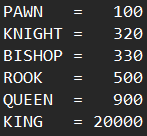
\includegraphics{figures/pieces_values.png}
      \captionof{figure}{Base values for the pieces}
      \label{fig:piecesValues}
    \end{minipage}
    \begin{minipage}{.49\textwidth}
      \centering
      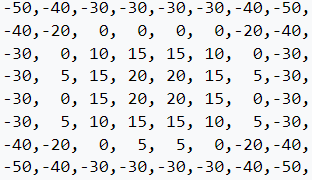
\includegraphics{figures/knight_value_table.png}
      \captionof{figure}{Knight value table}
      \label{fig:knightValueTable}
    \end{minipage}
\end{figure}

\begin{figure}[h]
    \centering
    \caption{King value tables}
    \begin{subfigure}{0.49\textwidth}
        \centering
        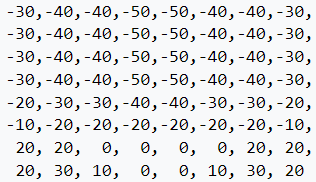
\includegraphics{figures/king_value_table_middlegame.png}
        \caption{King middlegame value table}
        \label{fig:kingValueTableMiddlegame}
    \end{subfigure}
    \begin{subfigure}{0.49\textwidth}
        \centering
        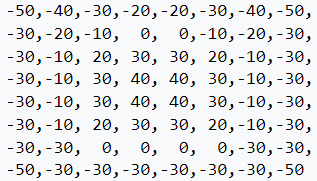
\includegraphics{figures/king_value_table_endgame.png}
        \caption{King endgame value table}
        \label{fig:kingValueTableEndgame}
    \end{subfigure}
\end{figure}

\subsection{Neural network}
\label{subsec:ch4sec3subsec2}

For the second evaluation function, I trained a neural network on master chess matches, which I will expand in a separate chapter.